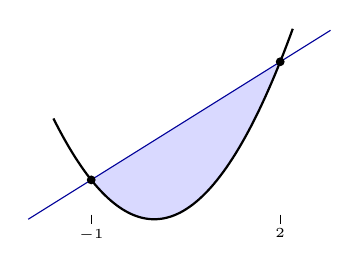
\begin{tikzpicture}[x=8mm,y=5mm]
\fill[blue!15] plot[domain=-1:2,samples=60] (\x,{\x+2}) -- plot[domain=2:-1,samples=60] (\x,{(\x)^2}) -- cycle;
\ax{-2}{3}{-0.6}{5}
\draw[thick,domain=-1.6:2.2,samples=80] plot (\x,{(\x)^2});
\draw[blue!60!black,domain=-2:2.8,samples=80] plot (\x,{\x+2});
\draw (-1,0.12)--(-1,-0.12); \node[below] at (-1,0){\tiny $-1$};
\draw (2,0.12)--(2,-0.12); \node[below] at (2,0){\tiny $2$};
\fill (-1,1) circle (1.6pt);
\fill (2,4) circle (1.6pt);
\end{tikzpicture}